\section{宣传}
由同学制作好推文之后,我们在朋友圈,98,朵朵等平台转发和宣传了我们的\href{https://v.xiumi.us/board/v5/70Xhf/619220060}{推文}。
\begin{figure}[H]
\centering
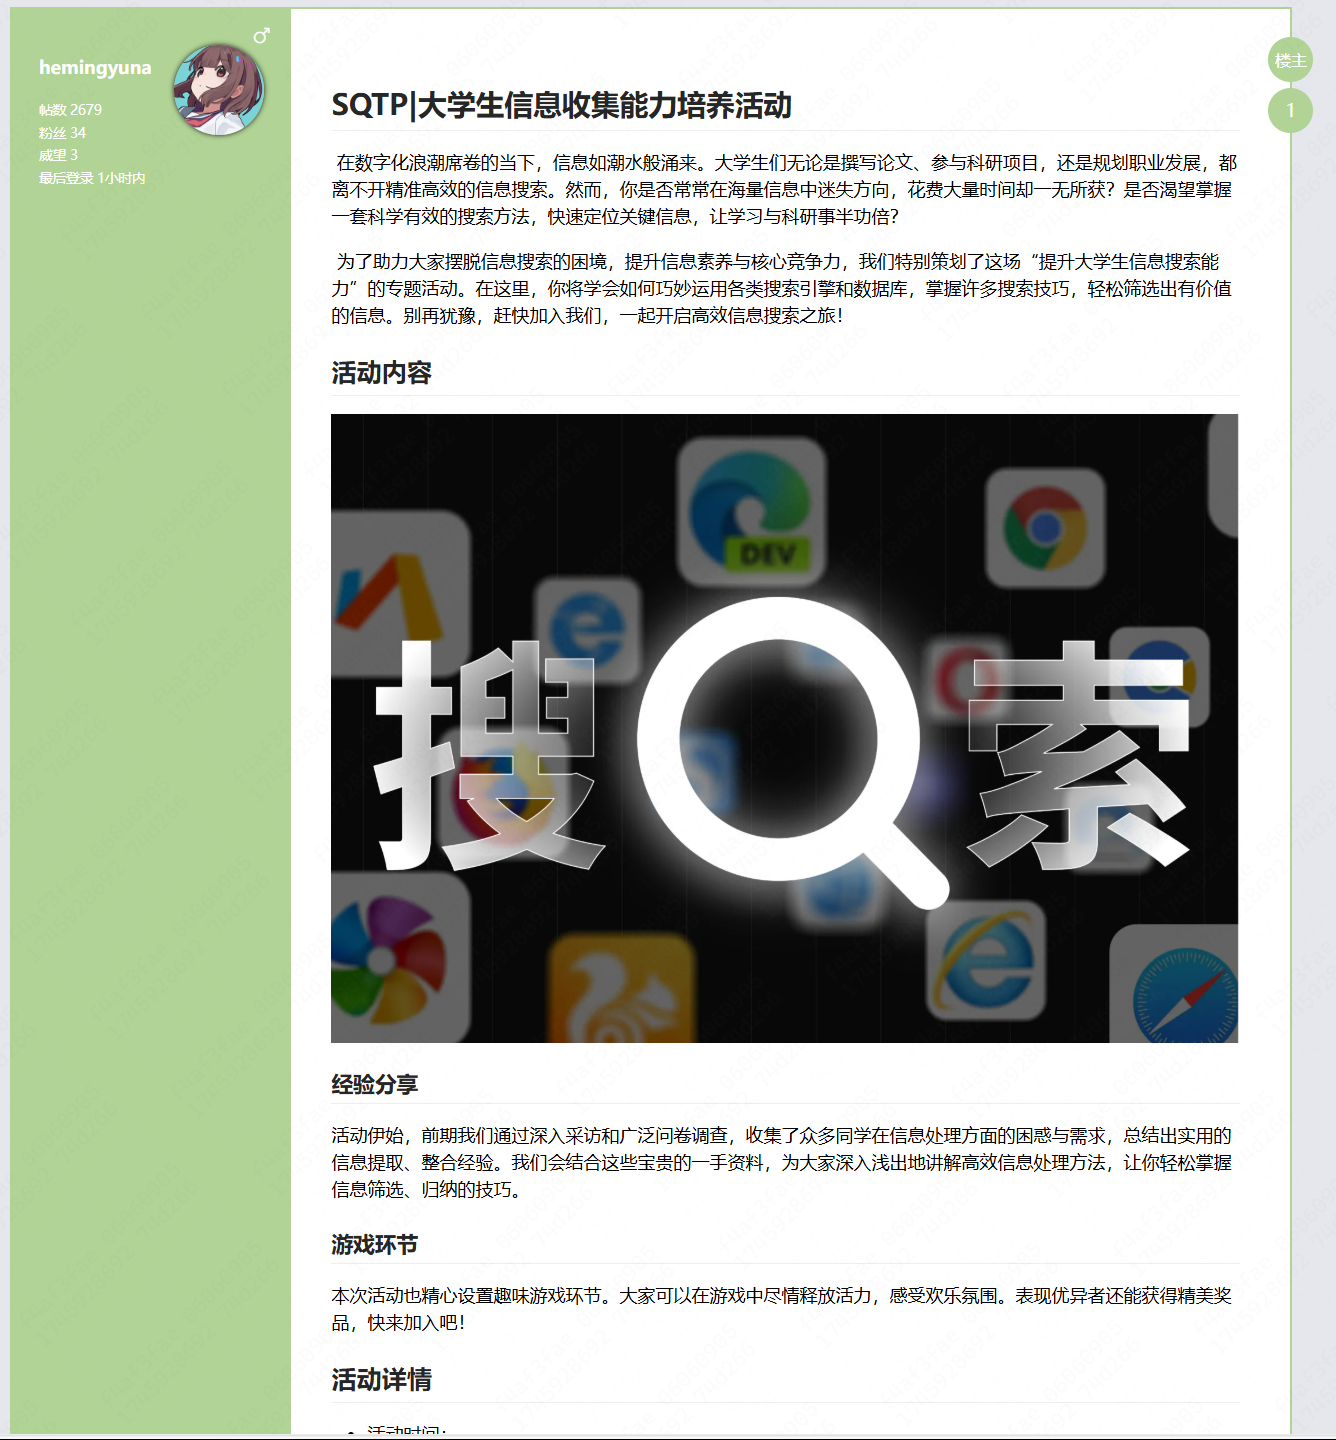
\includegraphics[width=.8\textwidth]{./figures/电脑端推文.png}

\includegraphics[width=.8\textwidth]{./figures/98宣传.png}
\caption{98推文及效果}
\end{figure}
\begin{figure}[H]
\centering

\includegraphics[width=.7\textwidth]{./resource/沙龙海报 .jpg}
\caption{活动海报}
\end{figure}
\section{宣讲会}
宣讲会基本按照手册编写顺序进行演讲,其中穿插了部分现场的案例演示与讲解。
\begin{figure}
    \centering
    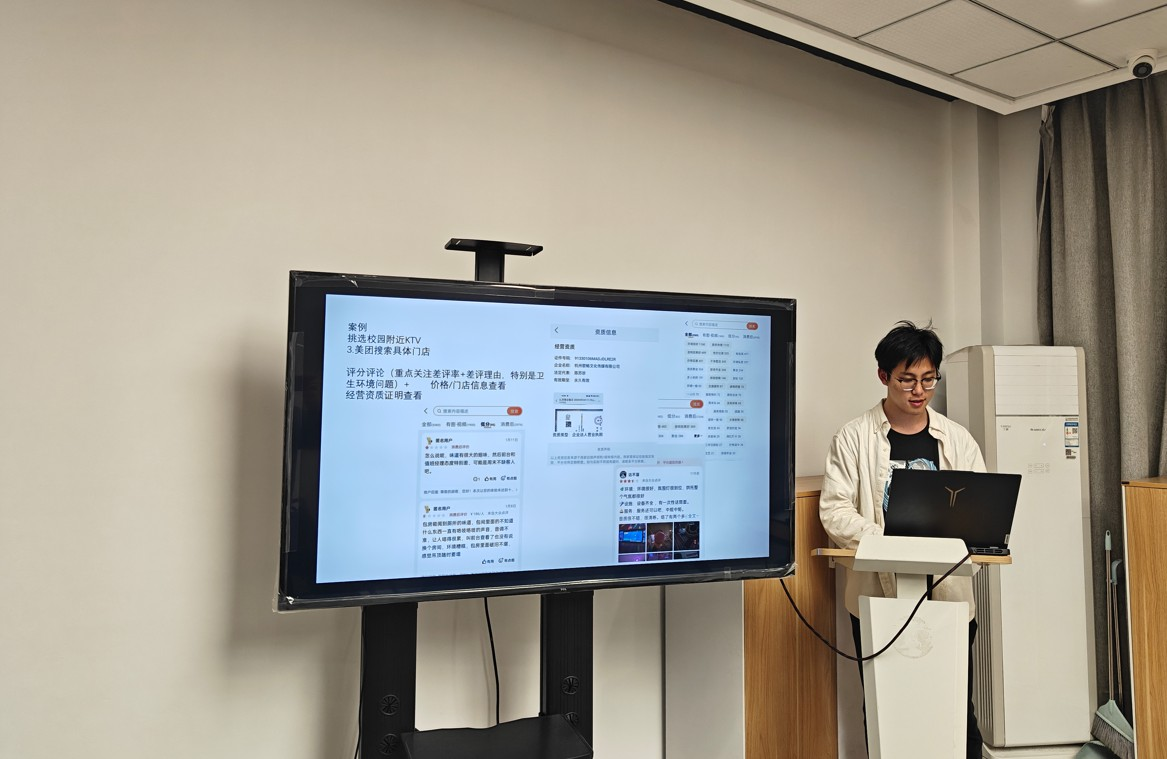
\includegraphics[width=.5\textwidth]{./figures/线下.jpg}
    \caption{线下宣讲}
\end{figure}
\section{网络迷踪信息搜索游戏}
\subsection{题目节选}
\begin{enumerate}
    \item 科研过程中遇到无法处理的实验数据时,会怎样处理
    \item 要写一篇课程论文,你会通过哪些途径完成你的论文
    \item 假如你是一个从未到过浙江大学的人,现在有一次机会可以来浙大游玩,你会怎样做攻略
    \item 你是一个不怎么会做饭的人,有一天爸妈都不在家,你又不想点外卖,会如何完成这顿饭的制作
    \item 突然电脑死机了,你会怎样解决这一问题
    \item 你和同学在某商城里寻找吃饭的地点。你会用什么途径寻找尽量好的餐厅?
    \item 3天后你就要大物小测了。你该如何寻找合适的复习资料?
    \item 允许使用电子设备搜索的课堂小测上,你该如何最快地找到尽可能对的答案?
    \item 选课时,你能列举3种获取课程信息的方式吗?
    \item 在qq等非正式平台看到了感兴趣的政治新闻,应该在哪里获取官方报道?
    \item 你准备保研,你应该去哪里查找上届保研录取分数?
\end{enumerate}
\begin{figure}
    \centering
    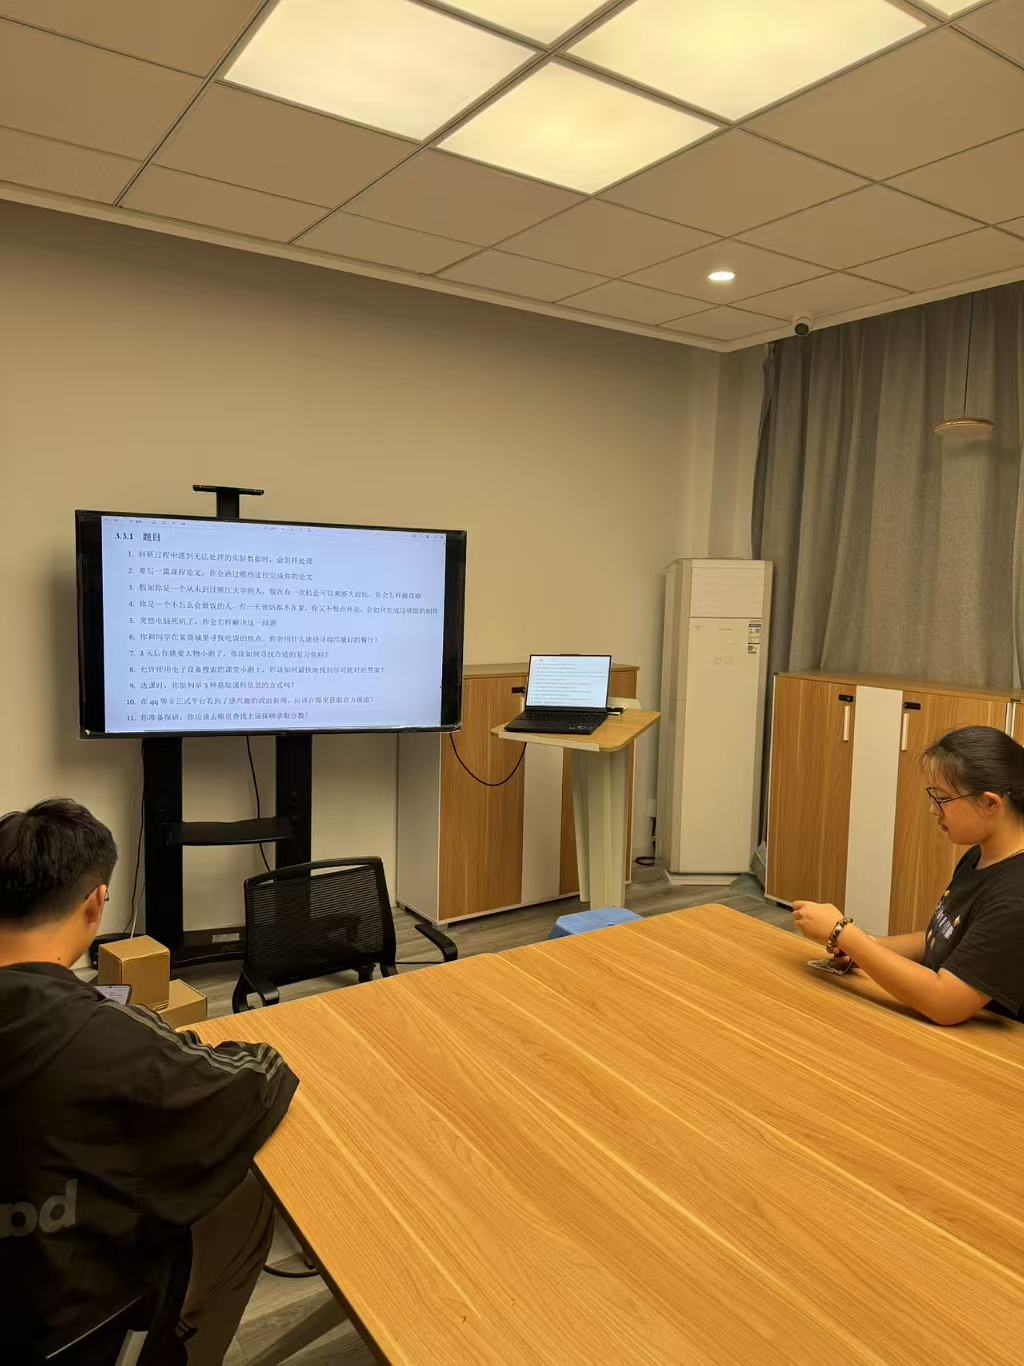
\includegraphics[width=.4\textwidth]{./figures/收集.jpg}
    \quad
    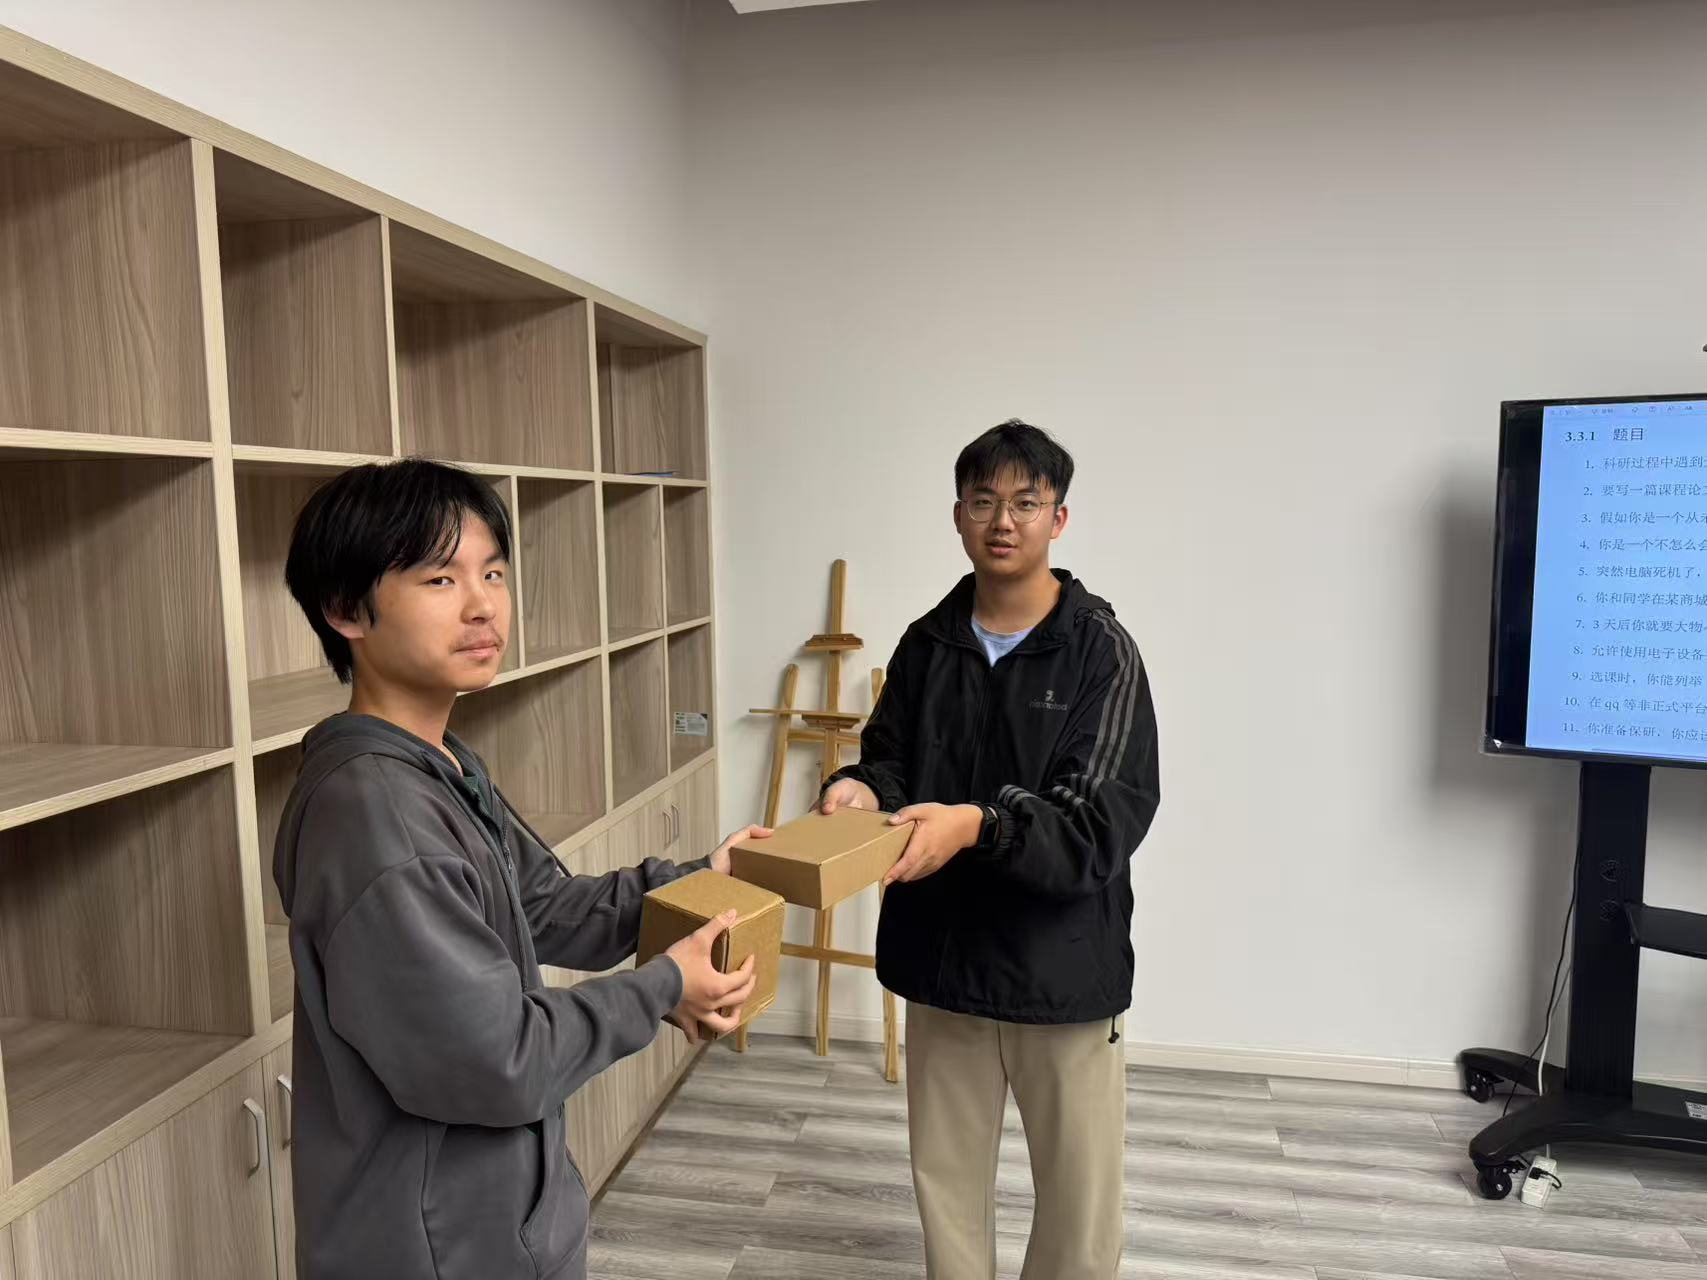
\includegraphics[width=.4\textwidth]{./figures/奖品发放.jpg}
    \caption{竞速信息收集与奖品发放}
\end{figure}
\subsection{反响}
关于``网络迷踪活动''同学们的反响:
\begin{notebox}
    ​参加网络迷踪游戏后,
    我深感这不仅是一场趣味横生的挑战,更是一次信息素养的实战演练。
    ​活动通过模拟真实的网络搜索场景,要求我们在海量信息中迅速提取有效线索,锻炼了我的观察力、逻辑思维和信息检索能力。
\end{notebox}
活动总结:

此次线下活动以“PPT宣讲会”与“网络迷踪信息搜索游戏”为核心,通过理论与实践结合的形式来提升大学生的信息检索能力与信息素养。
宣讲会围绕电子手册中科研、学习、生活三大场景的信息收集技巧展开,
结合案例演示与实时操作,深入解析关键词优化、数据库使用、多平台资源整合等方法,
帮助参与者构建结构化检索思维。
网络迷踪活动则创新性地将信息素养训练融入游戏机制,通过模拟真实搜索场景设计挑战题目,
要求参与者综合运用布尔逻辑检索等技巧,在限定时间内精准定位答案。
这种“寓教于乐”的形式不仅强化了理论知识的实际应用,还通过小礼品奖励机制激发参与热情,推动从被动接受信息到主动解决问题的思维转变。